\subsection{Información General}

La \textbf{Universidad Nacional de Ingeniería (UNI)} es una institución pública de educación superior fundada en 1876 bajo el nombre de Escuela Especial de Ingenieros de Construcción Civiles y de Minas. Se rige por la Ley Universitaria y su Estatuto institucional \cite{ley30220, estatuto2025}.

\paragraph{Actividad principal y servicios que ofrece}
Su actividad principal es la formación profesional en pregrado y posgrado en las áreas de ingeniería, ciencias y arquitectura. Además, realiza investigación científica, desarrollo tecnológico y actividades de apoyo a la sociedad.

Entre los principales servicios que brinda a su comunidad se encuentran:
\begin{itemize}
    \item \textbf{Servicios de formación académica:} Dictado de asignaturas teóricas y experimentales en aulas y laboratorios especializados, asesoría docente y acceso a bibliotecas físicas y digitales.
    \item \textbf{Servicios de soporte y registros:} Administración del historial académico, trámites documentarios y matrícula a través de la plataforma informática institucional.
    \item \textbf{Servicios de bienestar universitario:} Atención en medicina general y preventiva en el Centro Médico, cobertura del Fondo de Autoseguro Estudiantil, comedor universitario, programas deportivos y orientación psicopedagógica.
\end{itemize}

\paragraph{Público atendido}
La universidad atiende a estudiantes de pregrado y posgrado, egresados, investigadores y docentes. En este trabajo, el público directo son los estudiantes de pregrado de las escuelas profesionales de la Facultad de Ciencias que se inscriben cada semestre mediante el proceso de matrícula regular.

\paragraph{Ubicación geográfica}
El campus central de la Universidad Nacional de Ingeniería está ubicado en la Av. Túpac Amaru N.\textsuperscript{o} 210, en el distrito del Rímac, Lima, Perú. En este campus funcionan las once facultades de la universidad, incluida la Facultad de Ciencias, así como las oficinas administrativas centrales que participan en el proceso de matrícula.

% =========================================================================
% EVIDENCIA PENDIENTE POR EL USUARIO:
% Nombre del archivo esperado: images/mapa_ubicacion_uni.png
% Qué capturar: Captura de Google Maps u OpenStreetMap con la vista aérea
% o de plano del campus central de la UNI (Rímac), señalando el campus y
% preferentemente la Facultad de Ciencias o el acceso principal.
% =========================================================================
\begin{figure}[H]
    \centering
    \IfFileExists{images/mapa_ubicacion_uni.jpg}{%
        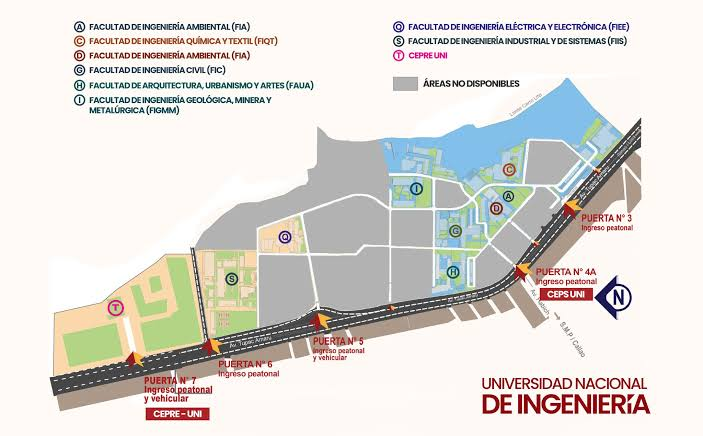
\includegraphics[width=0.85\textwidth]{images/mapa_ubicacion_uni.jpg}%
    }{%
        \fbox{\parbox{0.85\textwidth}{\centering\vspace{0.8cm}\textbf{[Figura pendiente: Plano o mapa de ubicación de la UNI]}\\\texttt{images/mapa\_ubicacion\_uni.jpg}\\{\small Ubicación del campus central en Av. Túpac Amaru 210, Rímac, destacando la Facultad de Ciencias.}\vspace{0.8cm}}}%
    }
    \caption{Ubicación geográfica del campus central de la Universidad Nacional de Ingeniería.}
    \label{fig:mapa_ubicacion_uni}
\end{figure}
